\section{Description du système}

\begin{figure}[h]
\begin{center}
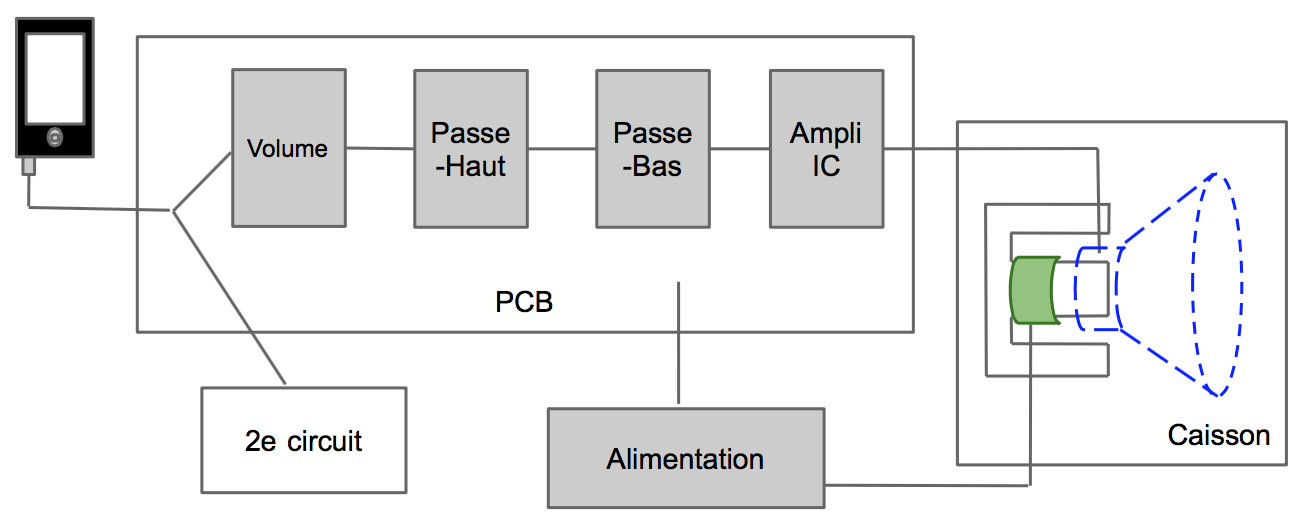
\includegraphics[width=\textwidth]{img/schemacomplet} 
\end{center}
\caption{Schéma général du système}		
\label{fig:schemacomplet}		
\end{figure}

Le système (voir figure~\ref{fig:schemacomplet}) est constitué de deux parties principales : le circuit imprimé (PCB) et l'enceinte. 
Ces deux parties ont été réalisées en double afin de pouvoir gérer un signal stéréo ou d'utiliser un des deux baffles principalement pour les aigus et l'autre pour les basses. Le circuit de ces deux hauts-parleurs est identique. Vous trouverez une copie du schéma électrique en annexe \ref{circuitcomplet}.
Le signal provenant du smartphone ou baladeur audio est transmis à la PCB grâce à une prise Jack 3.5 \milli\meter.
La PCB est composée de quatre parties principales :
\begin{itemize}
\item Une prise à laquelle est branché le câble jack, ce qui permet de séparer le signal et de l'envoyer aux deux circuits imprimés.
\item Un potentiomètre qui rend possible le réglage du volume.
\item Un filtre passe-haut et un filtre passe-bas, permettant respectivement de filtrer les basses et les aigus. Ces deux filtres sont alimentés en +15\,\volt \, et -15\,\volt \, par une source de tension continue.
\item Un amplificateur, permettant d'amplifier 50 fois le signal de sortie.
\end{itemize}
Le signal à la sortie de la PCB est envoyé vers la suite du système pour être converti en un mouvement mécanique : 
L'électroaimant (solénoïde fixe dans lequel circule du courant) génère un champ magnétique qui à son tour engendre une force mettant en mouvement la bobine mobile.~\footnote{Celle-ci est alimentée par une source de tension de laboratoire.}
Ses vibrations sont transmises à la membrane qui fait vibrer l'air et reproduit le son souhaité.
\textbf{PAS TERMINE}

Les 2 caissons sont pour leur part différents, un des 2 à plutôt été conçu pour les aigus, il s'agit d'un petit haut-parleur de type ouvert. Le second à été conçu pour les basses, il s'agit d'un plus gros haut-parleur de type bass-reflex.




